%!TEX root = documentation.tex

\chapter{Sensors}

\begin{figure}[ht]
    \centering
    \subfloat[Wind sensor from ThiesKlima]{\label{fig:windsensor} 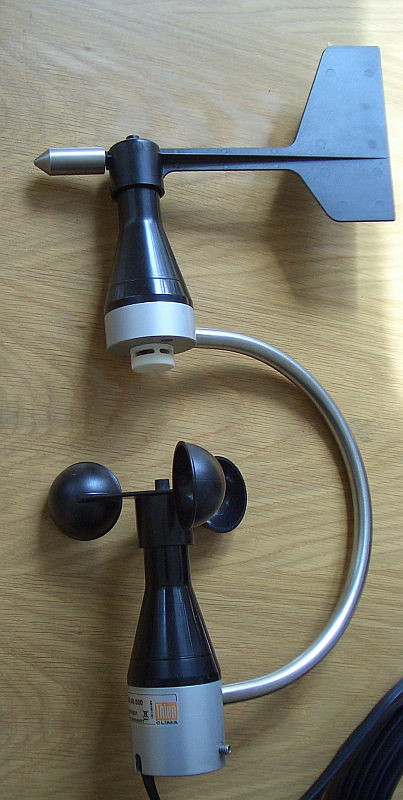
\includegraphics[width=0.4\linewidth]{graphics/windsensor.jpg}} 
    \qquad
    \subfloat[Dimensions of wind sensor]{\label{fig:windsensor_dim} 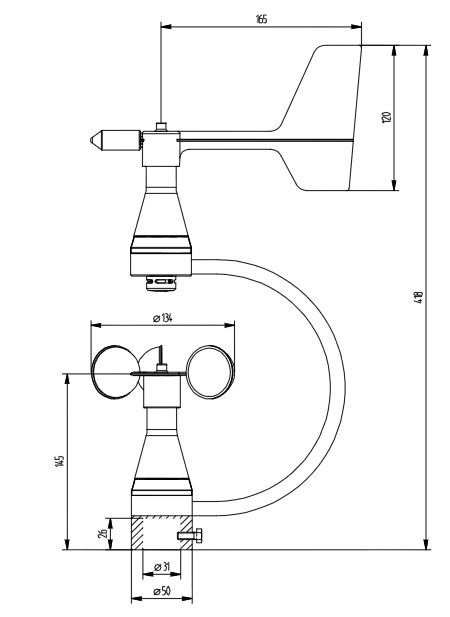
\includegraphics[width=0.5\linewidth]{graphics/windsensor_dim.jpg}}
    \qquad
    \label{view:windsensor1}
\end{figure}

For capturing the monitored parameters wind speed, wind direction and temperature, a product of ThiesKlima is used combining all needed sensors into one device. The connection between the sensor device and the microcontroller board is established by a 6-pin RJ-25 plug.

\begin{figure}[ht]
    \centering
    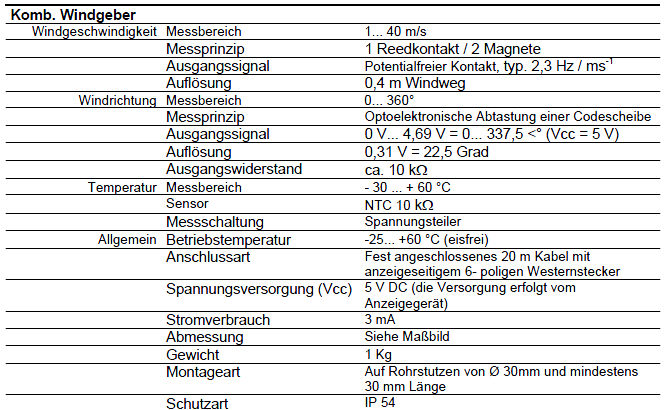
\includegraphics[width=0.9\linewidth]{graphics/windsensor_specs.jpg}
    \caption{Specification of wind sensor}
    \label{fig:windsensor_spec}
\end{figure}

\begin{figure}[ht]
    \centering
    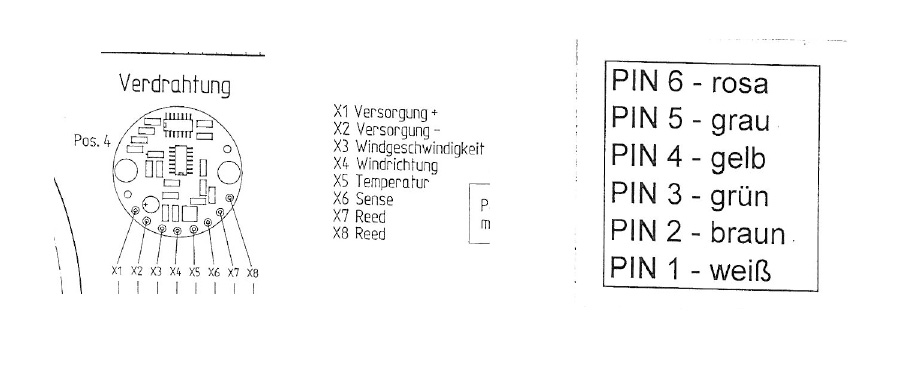
\includegraphics[width=0.8\linewidth]{graphics/windsensor_pinlayout.jpg}
    \caption{Pin layout of sensor plug}
    \label{fig:windsensor_pinlayout}
\end{figure}

\newpage